\subsection{Architecture Definition Verification}\label{sec:archVV}
The goal of architecture definition verification is to evaluate \progname{}'s
Module Guide (MG) for correctness, consistency, completeness, readability,
testability, and traceability. This corresponds to the design evaluation and
traceability analysis tasks in Section 9.3 of IEEE Std 1012-2016~\citep{vvIEEE}.

\paragraph{Method} The MG verification plan relies on peer review/document
inspection with the following stages:
\begin{enumerate}

    \item Preparation: Participants review the MG document with respect to
    their assigned role and goals (Table~\ref{tab:rolesMG})

    \item Meeting: Participants meet to discuss findings, potential issues, and
    proposed action plans to address them

    \item Rework: The MG author revises the document to address raised issues,
    guided by the proposed action plans

    \item Follow Up: Participants verify that raised issues have been addressed
    satisfactorily

\end{enumerate}

A recording device might be used to capture meeting proceedings in place of
physical note taking so that all participants can focus on the discussion.

Peer review/inspection begins when there is a new major version of the MG
document.

Peer review/inspection ends when reviewers agree that there are no issues that
will likely result in an extensive loss of confidence in \progname{} (e.g. an
unaddressed requirement).

\paragraph{Roles and Responsibilities} To assist in the achievement of their
assigned goals (Table~\ref{tab:rolesMG}) using peer review/document inspection:
\begin{itemize}

    \item Primary team members are responsible for ensuring that reviewers have
    the necessary materials, moderating the inspection process and reading
    through the MG document during the meeting(s)

    \item Secondary and tertiary members are reviewers whom are responsible for
    reviewing the MG document prior to the meeting so that they are prepared to
    discuss it with the team

\end{itemize}

\paragraph{Inputs}
\begin{itemize}

    \item Module Guide for \progname{}: A Computational Model of Emotion for
    Enhancing Non-Player Character Believability in Games

    \item Software Requirements Specification for \progname{}: A Computational
    Model of Emotion for Enhancing Non-Player Character Believability in Games

    \item Review guide for \progname{}'s MG
    (Appendix~\ref{appendix:archInspection})

\end{itemize}

\paragraph{Outputs}
\begin{itemize}

    \item Objective evidence to assess the verification of the MG

    \item Objective evidence that the architecture design is complete, correct,
    accurate, and testable

    \item Objective evidence that the architecture design is realizable

    \item Objective evidence that the architecture design satisfies the
    requirements described in \progname{}'s Software Requirements Specification
    (SRS)

    \item Objective evidence that the MG is readable

    \item Input to Master Test Report (MTR)

\end{itemize}

\paragraph{Estimated Completion Time} One (1) week

\begin{figure}[!h]
    \centering
    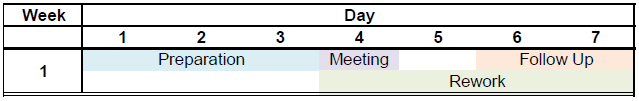
\includegraphics[width=0.9\linewidth]{figures/MG_Schedule.png}
\end{figure}